\documentclass{article}[18pt]
\usepackage{../../../../../format}
\lhead{CSys - Databases}
\usepackage{minted}

\begin{document}
\begin{center}
\underline{\huge Distributed Architectures and DBMS}
\end{center}
\section{Multi User DBMS Architectures}
\begin{itemize}
	\item So far we have seen this model of interaction between end users and the database
	\begin{itemize}
		\item One central DBMS
		\item Users interact with DBMS using an application program
	\end{itemize}
	\item Several issues still need clarification:
	\begin{itemize}
		\item Is the DBMS on the end user's computer
		\item How are the users connected to the DBMS?
		\item Do we have one or more DBMS?
		\item Which computations are performed where?
		\item Is the database stored in one or many places
	\end{itemize}
	\item Teleprocessing Architecture:
	\begin{itemize}
		\item The traditional (and most basic) architecture
		\item One computer with a single CPU
		\item Many (end-user) terminals all cabled to the central computer
		\item The terminal sends messages to the central computer
		\item All data processing in the central computer
		\item This puts tremendous burden on the central computer leading to decreased performance
	\end{itemize}
	\item Nowadays, the trend is towards downsizing
	\begin{itemize}
		\item Replace expensive mainframe computers with cost-effective networks of personal computers
		\item Achieve the same/better 
	\end{itemize}
\end{itemize}
\section{File-Server architecture}
Processing is distributed around a computer network
\begin{itemize}
	\item Typically through a LAN
	\item One central file-server
	\item Every workstation has its own DBMS and its own user application
	\item Workstations request files they need from the file server
	\item File server acts like a "shared hard disk" (it has no DBMS)
\end{itemize}
\begin{minted}{sql}
SELECT fName, IName
FROM Branch b, Staff s
WHERE b.branchNo=s.branchNo AND b.street='163 Main St.'
\end{minted}
\begin{itemize}
	\item The file-server has no knowledge of SQL - the user's DBMS has to request the whole tables Branch, Staff
	\item Therefore:
	\begin{itemize}
		\item Very large amount of network traffic (the tables may be huge)
		\item A full copy of the DBMS required on each workstation
		\item Concurrency/recovery/integrity control is more difficult since multiple DBMSs access the same files simultaneously
	\end{itemize}
	\item The solution to these problems is a client-server architecture
\end{itemize}
\section{Client-Server architecture}
\begin{itemize}
	\item Client - Requires some resource
	\item Server - provides the resource
	\item Client/server are not always in the same machine/place
	\item Two-tier architecture
	\begin{itemize}
		\item Tier 1 (client): responsible for the presentation of data to the user
		\item Tier 2 (server): responsible for supplying data services to the user
	\end{itemize}
	\item Typical Procedure:
	\begin{itemize}
		\item User gives a request to the client
		\item Client generates SQL query and sends it to the server
		\item Server accepts, processes the query and sends the result to the client
		\item Client formats the result for the user
	\end{itemize}
	\item Many advantages:
	\begin{itemize}
		\item Increased performance: many client CPUs
		\item Reduced Hardware Costs: only the server needs increased storage and computational power
		\item Reduced communication costs: less data traffic (not unnecessary are transmitted)
	\end{itemize}
	\item Database is still centralized - not a distributed database
\end{itemize}
\section{Three-Tier Client-Server Arch}
\begin{itemize}
	\item In modern system: 100s/1000s of users - need for increased enterprise 
	\item Main problem of the client that prevent scalability - a "fat client" (many users) requires extensive resources on disk space/RAM/CPU power
	\item A new variant on the client server architecture
	\begin{itemize}
		\item Three layers, potentially running on different platforms
		\item First Tier: UI later (on end user's computer)
		\item Second Tier: application server (connects to many users)
		\item Third Tier: database server (contains DBMS, communicates with the application server)
		\item "Thin clients" - increased performance of user's computer
	\end{itemize}
	\item Best example for a client: internet browser
	\item Advantages:
	\begin{itemize}
		\item Smaller hardware cost for "thin clients"
		\item Easier application maintenance (centralized in one tier)
		\item Easier to modify/replace one tier without affecting others
		\item Easier load balancing between the different tiers
		\item Maps naturally to web applications
	\end{itemize}
	\item It can be extended
	\begin{itemize}
		\item Separation of tasks into $n$ intermediate tiers for increased flexibility and scalability 
	\end{itemize}
\end{itemize}
\section{Distributed DBMS}
\begin{itemize}
	\item So far we have seen centralized database systems
	\begin{itemize}
		\item single database, located at one site
		\item Controlled by one DBMS
	\end{itemize}
	\item We can improve database performance:
	\begin{itemize}
		\item Using networks of computers (decentralized approach)
		\item It mirrors the organizational structure:
		\begin{itemize}
			\item Logically distributed into divisions, departments, projects...
			\item Physically distributed into offices, flats, units, factories...
		\end{itemize}
	\end{itemize}
	\item Main targets
	\begin{itemize}
		\item Make all data accessible to all units
		\item Store the data proximate to the location where it is most frequently used
		\item Full functionality and efficiency
	\end{itemize}
	\item Distributed Database
	\begin{itemize}
		\item A logically interrelated collection of shared data physically distributed over a network
	\end{itemize}
	\item Distributed DBMS (DDBMS)
	\begin{itemize}
		\item The software system that can manage the distributed database
		\item It makes the distribution transparent (invisible) to users
	\end{itemize}
	\item In a DDBMS
	\begin{itemize}
		\item A single logical database, which is split into fragments
		\item Each fragment is stored on one (or more) computers, under the control of a separate DBMS
		\item All of these computers are connected by a communications network
		\item Sites have local autonomy: independent processing of local data (via local applications)
		\item Sites have access to global applications (to process data fragments stored on other computers)
	\end{itemize}
	\item Not all sites have local applications/local data
	\item All sites have access to global applications
	\item Data fragments may be replicated in more sites (data consistency must be considered)
\end{itemize}
\begin{center}
	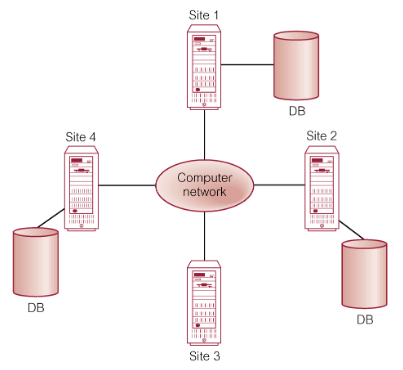
\includegraphics[scale=0.7]{Distributed}
\end{center}
\section{Distributed processing vs Distributed DBMS}
Distributed processing:
\begin{itemize}
	\item A centralized database that is accessed over a computer network
	\item For example: the client server architecture
	\item This is not the same as a distributed DBMS
\end{itemize}
\begin{center}
	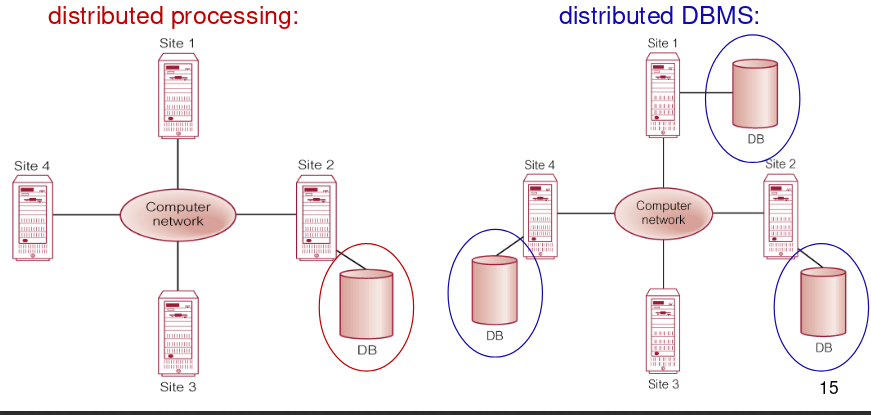
\includegraphics[scale=0.7]{processing}
\end{center}
\section{Design of a distributed DBMS}
In addition to ER modelling, we have to consider also:
\begin{itemize}
	\item Fragmentation:
	\begin{itemize}
		\item How to break a relation into fragments
		\item Fragments can be horizontal/vertical/mixed
	\end{itemize}
	\item Allocation: 
	\begin{itemize}
		\item How fragments are allocated at the several sites
		\item Aim is to reach an "optimal" distribution (efficient, reliable,...)
	\end{itemize}
	\item Replication
	\begin{itemize}
		\item Which fragments are stored in multiple sites (and which sites)
	\end{itemize}
\end{itemize}
Choices for Fragmentation and Allocation:
\begin{itemize}
	\item Based on how the database is to be used
	\item Quantitative and Qualitative information is used
\end{itemize}
\begin{itemize}
	\item Quantitative information (mainly for fragmentation)
	\begin{itemize}
		\item The frequency with which specific transactions are run
		\item The (usual) sites from which transactions are run
		\item Desired performance criteria for the transactions
	\end{itemize}
	\item Qualitative information (mainly for allocation):
	\begin{itemize}
		\item The relations/attributes/tuples being accessed
		\item The type of access (read/write)
	\end{itemize}
	\item Strategic objectives for the choices about the fragments
	\begin{itemize}
		\item Locality of reference
		\begin{itemize}
			\item Data to be stored close to where it is used
			\item If a fragment is used at several sites then replication is useful
		\end{itemize}
		\item Reliability and availability
		\begin{itemize}
			\item Improved by replication
			\item If one site fails, there are other fragment copies available
		\end{itemize}
	\end{itemize}
\end{itemize}
Further strategic objectives
\begin{itemize}
	\item Acceptable performance
	\begin{itemize}
		\item Bad allocation results in "bottleneck" effects (a site receives too many requests so has bad performance)
		\item Also: Bad allocation caused underutilized resources
	\end{itemize}
	\item Cost of storage capacities
	\begin{itemize}
		\item Cheap mass storage to be used at sites, whenever possible
		\item This must be balanced against locality of reference
	\end{itemize}
	\item Minimal communication costs
	\begin{itemize}
		\item Minimum retrieval costs when max locality of reference, or when each site has its own copy of data
		\item But when replicated data is updated
		\begin{itemize}
			\item All copies of this data must be updated
			\item Increased network traffic/communication costs
		\end{itemize}
	\end{itemize}
\end{itemize}
Four alternative strategies for the placement of data
\begin{itemize}
	\item Centralized
	\begin{itemize}
		\item Single database and DBMS
		\item Stored at one site with users distributed across the network
		\item Not distributed
	\end{itemize}
	\item Partitioned
	\begin{itemize}
		\item Database partitioned into disjoint fragments
		\item Each data item assigned to exactly one site (no replication)
	\end{itemize}
	\item Complete replication
	\begin{itemize}
		\item Complete copy of the database at each site
	\end{itemize}
	\item Selective replication
	\begin{itemize}
		\item Combination of partitioning, replication and centralization
	\end{itemize}
\end{itemize}
\begin{center}
	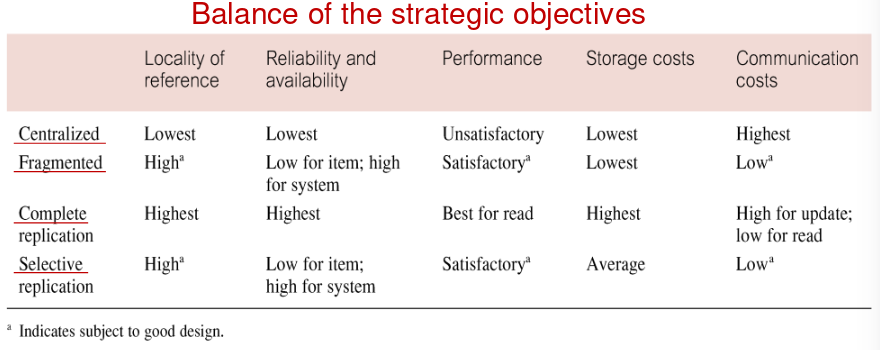
\includegraphics[scale=0.7]{Strategies}
\end{center}
Three correctness rules for the partitioned placement
\begin{enumerate}
	\item Completeness
	\begin{itemize}
		\item If relation R is decomposed into fragments $R_1,R_2,...R_n$ each data item in R must appear in at least one fragment $R_i$
	\end{itemize}
	\item Reconstruction
	\begin{itemize}
		\item It must be possible to define a relational algebra expression that can reconstruct R from its fragments
	\end{itemize}
	\item Disjointness
	\begin{itemize}
		\item If a data item appears in fragment $R_i$, it should not appear in any other fragment
		\item Exception for vertical fragmentation: primary key attributed must be repeated for the reconstruction
	\end{itemize}
\end{enumerate}
\section{Fragmentation}
Three main types of fragmentation
\begin{enumerate}
	\item Horizontal
	\begin{itemize}
		\item A subset of the tuples of the relation
	\end{itemize}
	\item Vertical
	\begin{itemize}
		\item A subset of the attributes of the relation
	\end{itemize}
	\item Mixed
	\begin{itemize}
		\item A vertical fragment that is then horizontally fragmented
		\item Or a horizontal fragment that is then vertically fragmented
	\end{itemize}
\end{enumerate}
\subsection{Horizontal fragmentation}
\begin{itemize}
	\item Assume there exist two property types: 'Flat' and 'House'
	\item We have a relation R with all properties for rent
	\item The horizontal fragmentation of R (by property type) is
	$$P_1=\sigma_{type='House'}(PropertyForRent)$$
	$$P_2=\sigma_{type='Flat'}(PropertyForRent)$$
	\item This fragmentation may be useful e.g. if we have separate applications dealing with flats/houses
	\item And it is correct
	\begin{itemize}
		\item \textbf{Completeness}: Each tuple is in either $P_1$ or in $P_2$
		\item \textbf{Reconstruction}: $R$ can be constructed from the fragments $P_1,P_2$
		$$R=P_1\cup P_2$$
		\item \textbf{Disjointness}: There is no property that is both 'flat' and 'house'
	\end{itemize}
\end{itemize}
\subsection{Vertical Fragmentation}
\begin{itemize}
	\item For every staff member in a company
	\begin{itemize}
		\item The payroll department requires: \texttt{staffNo, position, sex, salary}
		\item The personnel department requires: \texttt{staffNO, fName, DOB, branchNo}
	\end{itemize}
	\item We have a relation Staff with all staff members
	\item For this example, the vertical fragmentation of staff is:
	$$S_1=\Pi_{\text{staffNo, position, sex, salary}}(Staff)$$
	$$S_2=\Pi_{\text{staffNo, Name, DOB, branchNo}}(Staff)$$
	\item Both fragments include the primary key staffNo to allow reconstruction of Staff from $S_1$ and $S_2$
	\item This fragmentation is useful
	\begin{itemize}
		\item The fragments are stored at the departments that are needed
		\item Performance for every department is improved (as the fragment is smaller than the original relation Staff)
	\end{itemize}
	\item This fragmentation is correct
	\begin{itemize}
		\item \textbf{Completeness}
		\begin{itemize}
			\item The primary key \texttt{staffNo} belongs to both $S_1$ and $S_2$
			\item Each other attribute is either in $S_1$ or in $S_2$
		\end{itemize}
		\item \textbf{Reconstruction}
		\begin{itemize}
			\item R can be constructed from the fragments $S_1,S_2$ using the natural join operation
		\end{itemize}
		$$Staff=S_1\bowtie S_2$$
		\item \textbf{Disjointness}
		\begin{itemize}
			\item The fragments are disjoint except the primary key (which is necessary for the reconstruction)
		\end{itemize}
	\end{itemize}
\end{itemize}
\section{Advantages and Disadvantages of a distributed DBMS}
Advantages
\begin{itemize}
	\item Reflects organizational structure
	\item Improves share-ability and local autonomy
	\item Improved availability and reliability 
	\item Improved performance
	\item Smaller hardware cost
	\item Scalability
\end{itemize}
Disadvantages
\begin{itemize}
	\item Complexity
	\item Higher maintenance cost
	\item Security
	\item Integrity control more difficult
	\item Design more complex
	\item Lack of experience in the industry
\end{itemize}


\end{document}